% 
% Annual CCN conference
% Sample LaTeX Two-Page Summary -- Proceedings Format
% based on the prior cognitive science style file

% Original : Ashwin Ram (ashwin@cc.gatech.edu)       04/01/1994
% Modified : Johanna Moore (jmoore@cs.pitt.edu)      03/17/1995
% Modified : David Noelle (noelle@ucsd.edu)          03/15/1996
% Modified : Pat Langley (langley@cs.stanford.edu)   01/26/1997
% Latex2e corrections by Ramin Charles Nakisa        01/28/1997 
% Modified : Tina Eliassi-Rad (eliassi@cs.wisc.edu)  01/31/1998
% Modified : Trisha Yannuzzi (trisha@ircs.upenn.edu) 12/28/1999 (in process)
% Modified : Mary Ellen Foster (M.E.Foster@ed.ac.uk) 12/11/2000
% Modified : Ken Forbus                              01/23/2004
% Modified : Eli M. Silk (esilk@pitt.edu)            05/24/2005
% Modified : Niels Taatgen (taatgen@cmu.edu)        10/24/2006
% Modified : David Noelle (dnoelle@ucmerced.edu)     11/19/2014
% Modified : Konrad Kording (koerding@gmail.com)     2/15/2017
% Modified : Thomas Naselaris (tnaselar@gmail.com)   3/18/2022

\documentclass[10pt,letterpaper]{article}

\usepackage{ccn}
\usepackage{pslatex}
\usepackage{apacite}
\usepackage{graphicx}
\usepackage{caption}
\usepackage{natbib}
\usepackage{float}

\usepackage{hyperref}       % hyperlinks
\usepackage{url}            % simple URL typesetting
\usepackage{booktabs}       % professional-quality tables
\usepackage{amsfonts}       % blackboard math symbols
\usepackage{nicefrac}       % compact symbols for 1/2, etc.
\usepackage{microtype}      % microtypography
\usepackage{xcolor}         % colors
\usepackage{amsmath}
\usepackage{amssymb}
\usepackage{mathtools}
\usepackage{amsthm}
\usepackage{graphicx}
\usepackage{svg}
\usepackage[labelfont=bf, margin=0.8cm, font=sf]{caption}
% \usepackage[margin=0.5in]{geometry}

\title{Title Here: Something that summarises the work}
 
\author{{\large \bf Author 1 } \\ University of the Witwatersrand, 1 Jan Smuts Ave,\\ Braamfontein, Johannesburg, 2000, South Africa
  \AND {\large \bf Author 2 } \\ University of the Witwatersrand, 1 Jan Smuts Ave,\\ Braamfontein, Johannesburg, 2000, South Africa
  \AND {\large \bf Author 3} \\ University of the Witwatersrand, 1 Jan Smuts Ave,\\ Braamfontein, Johannesburg, 2000, South Africa}


\begin{document}

\maketitle
\phantom{.}
\newpage
\phantom{.}
\newpage
\section{Abstract}
{
\bf
\looseness=-1
Roughly 20 lines. It should follow the format of the paper where each section is summarised as a sentence (not a fixed rule but a bit of a heuristic).
}
\begin{quote}
\small
\textbf{Keywords:} 
3 Words or phrases that give the main categories or topics of the work
\end{quote}

\section{Introduction} \label{Intro}
\looseness=-1
Describe the general problem, motivate why it is important to solve or understand better, outline what you do in the abstract, etc. Because this is a short document you do not need to have as elaborate of a throw-forward as you usually would but some description of the document structure could help. You also don't have to give bullet points of your contributions like usual, but you do need to be clear on what you do and why it should matter. If you include any figures throughout the abstract, please ensure that you reference them in the text. For example, I have included Figure~\ref{fig:wave}.

\subsubsection{Background}
\looseness=-1
Sometimes you may include subsections to make your text more structured. Since you don't have a lot of space you need to prioritise putting as much background in as you case without wasting space. So it will probably come as part of the Introduction (Section~\ref{Intro}) to avoid restating things.

% \setlength{\belowcaptionskip}{-2pt}
% \begin{wrapfigure}[34]{L}{0.45\textwidth}
\setlength{\belowcaptionskip}{-15pt}
\begin{figure}[h!]
  \captionsetup{margin=0.0in, font=sf}
  \begin{minipage}{\linewidth}
  \centering
    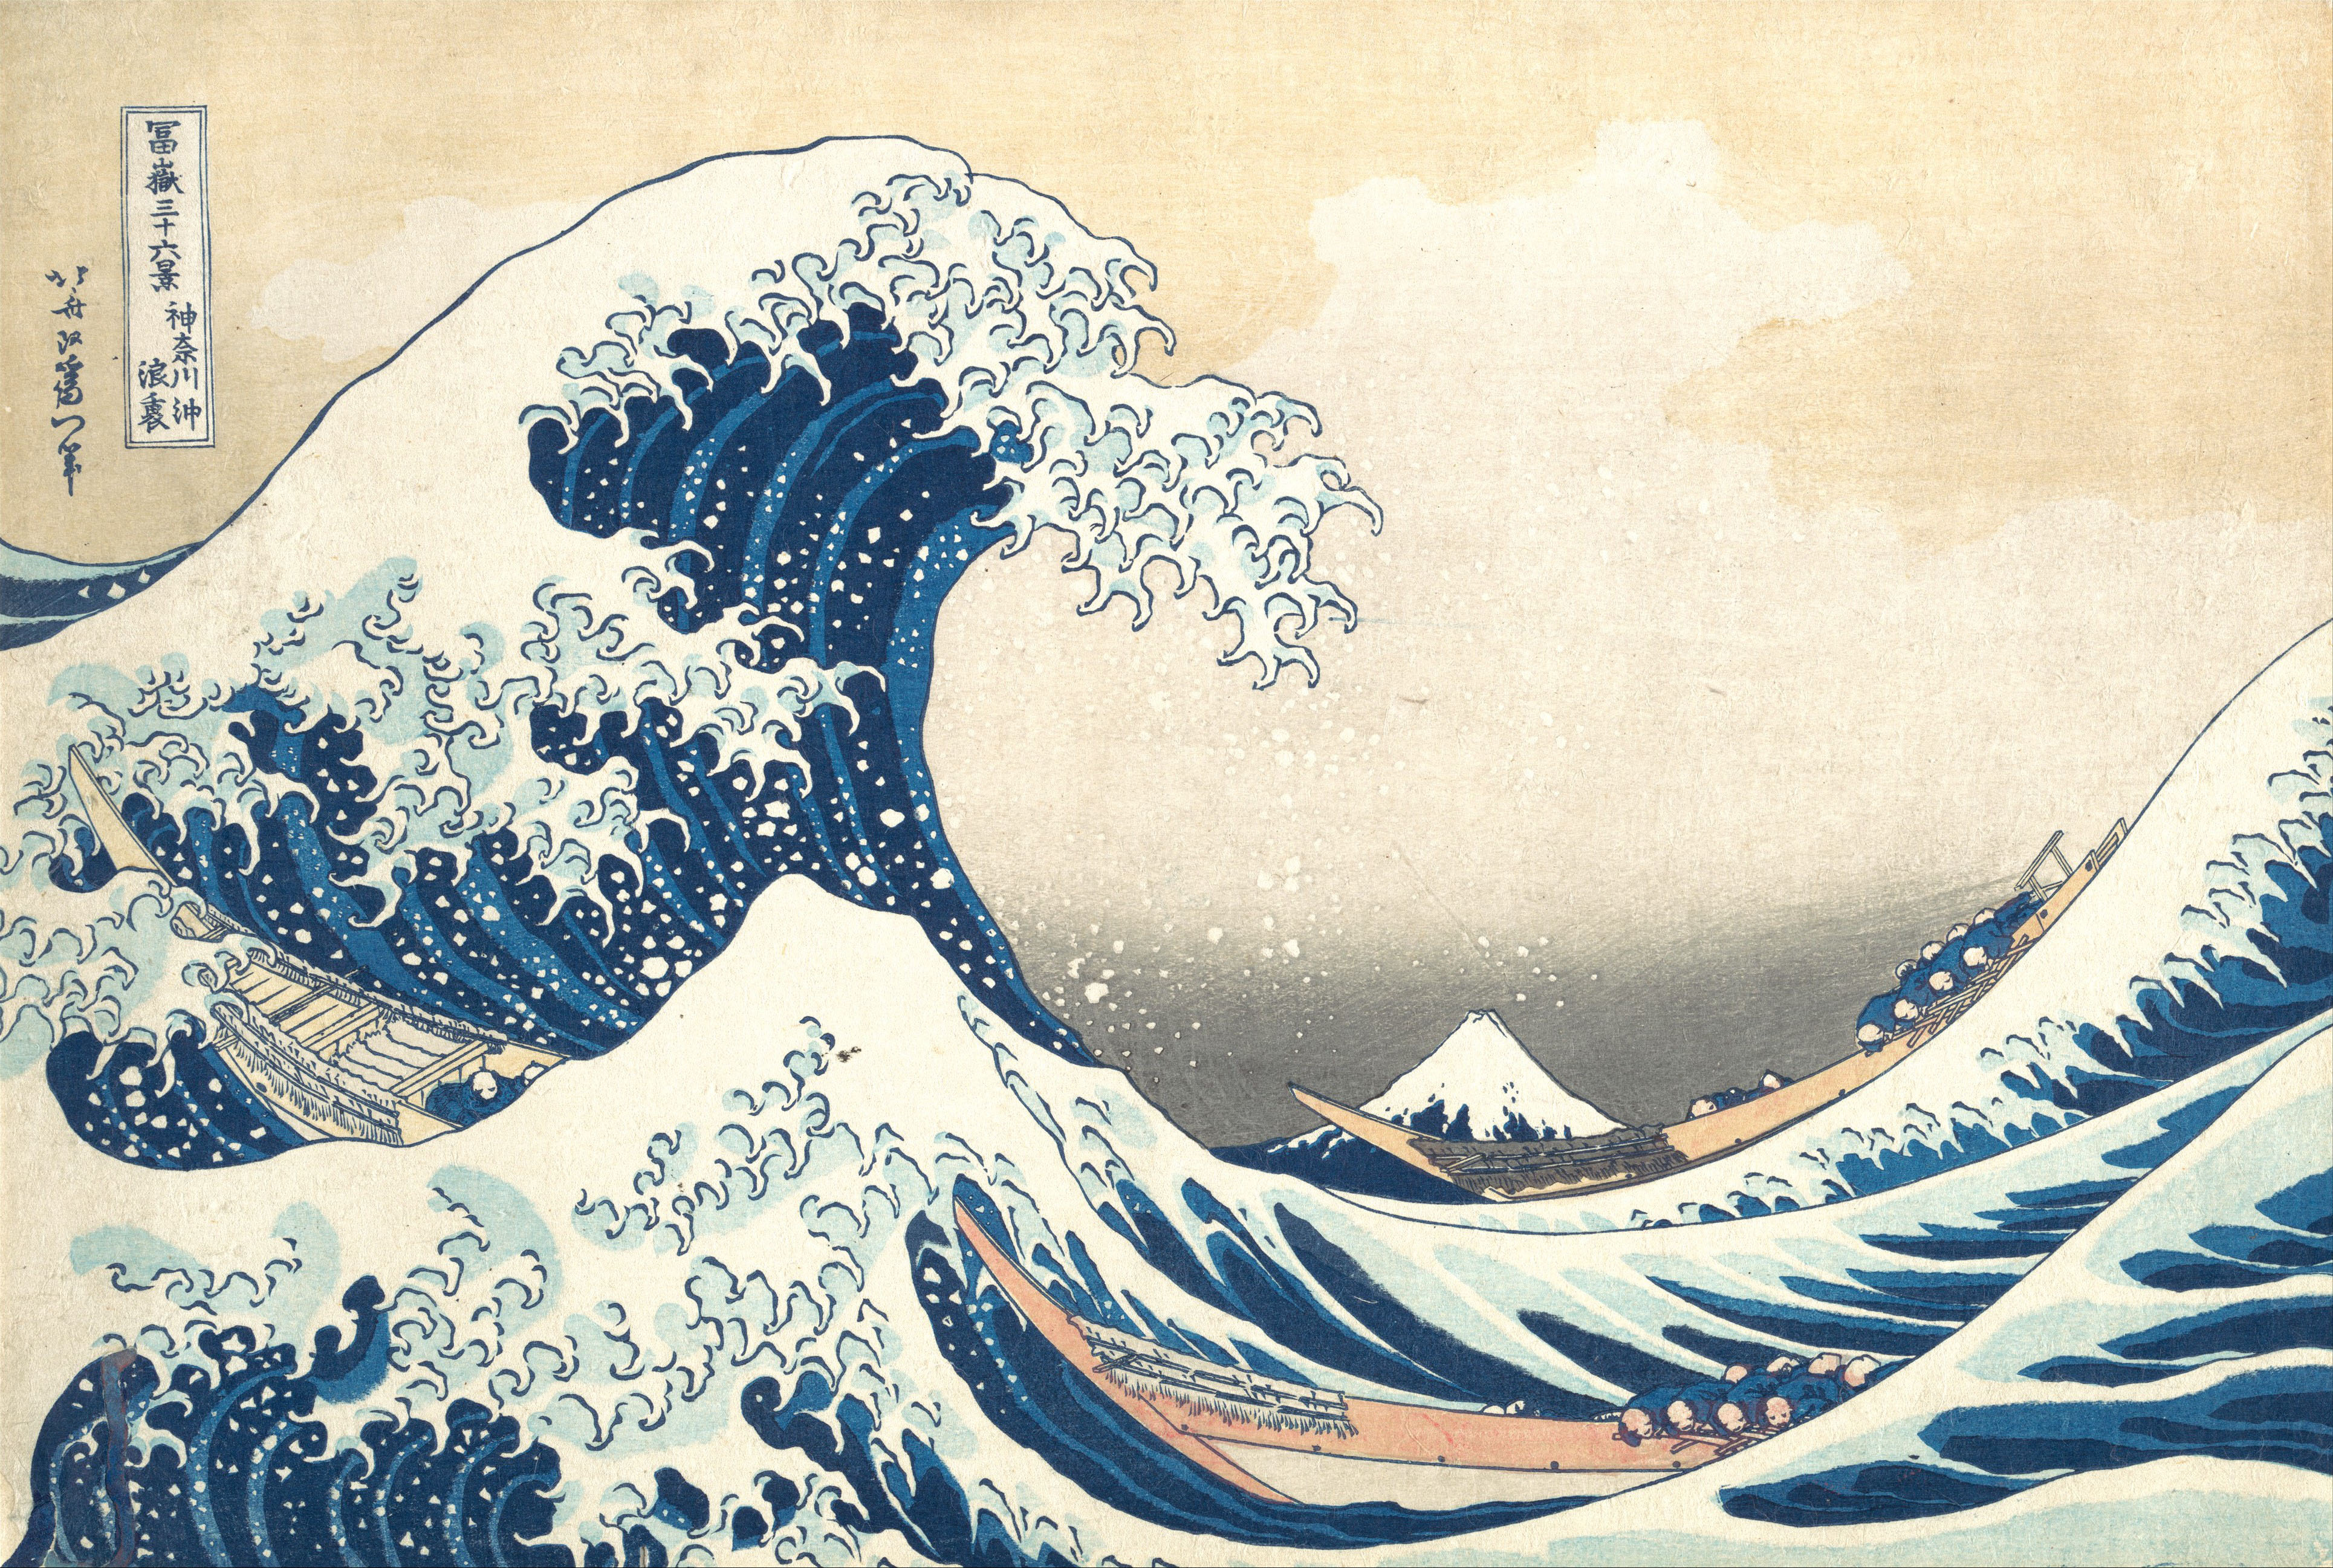
\includegraphics[width=1.0\linewidth]{images/image.jpeg}
  \end{minipage}
  \caption{\looseness=-1 Describe what the image shows. Do not just give a short statement about it -- it is not alternate text like an html image would have. Actually tell the reader the point of the image and where they should look. For example: ``The Great Wave off Kanagawa by Hokusai. This is Devon's favourite painting (although technically it is a print) due largely to the fact that it uses Prussian blue which gives the waves their distinctive colour \citep{smith2005hokusai}. Please remember that ``citep'' puts the citation in parenthesis (as you just saw) and ``citet'' is for in-text citations like \citet{smith2005hokusai}. It is easy to remember ``p'' for ``parenthesis'' and ``t'' for ``text''.}
  \label{fig:wave}
% \end{wrapfigure}
% \setlength{\belowcaptionskip}{0pt}
\end{figure}
\setlength{\belowcaptionskip}{0pt}

\section{Methods}
Describe your experiments and model. Try be clear how all of the design decisions (for both experiment and model) serve to answer the research question or provide a point. Make sure your experiments are controlled properly and that any phenomena are measurable or interpretable if you aim to draw conclusions from them.

\section{Results}
\looseness=-1
Describe your findings and present the outcomes or output from your experiments. Remember to reference any tables in the text too. For example, I included Table~\ref{tab:nonlin} as an example. Note that, typically we put table captions at the top and figure captions at the bottom. This is just a standard our field has settled into. This is not mandatory to follow here

\setlength{\belowcaptionskip}{-7pt}
\begin{table}[h!]
\centering
\captionsetup{font=sf, width=0.95\linewidth, skip=7pt}
\caption{\looseness=-1 Example table showing some very important results. We note that Linear and ReLU at $n=0$ has high error across both level which vanish for level 1 by the end of training ($n=200$). Importantly we find no level 4 improvement throughout training.}
\begin{tabular}{|c|c|c|} 
 \hline
 Model & \multicolumn{1}{|p{2cm}|}{\centering Level 1 Error\\ (Percentage)} & \multicolumn{1}{|p{2cm}|}{\centering Level 4 Error\\ (Percentage)} \\
 \hline\hline
 Linear; $n=0$ & 58.25 & 79.88 \\ 
 \hline
 Linear; $n=200$ & 0.0 & 62.50\\
 \hline
 ReLU; $n=0$ & 51.50 & 84.50 \\ 
 \hline
 ReLU; $n=200$ & 2.75 & 62.50 \\
 \hline
\end{tabular}
\label{tab:nonlin}
\end{table}
\setlength{\belowcaptionskip}{0pt}

\section{Discussion}
Take a broader perspective of your results and recontextualise them in terms of the field and your community. Your research should aim to be helpful to your community and you will stand better chances of gaining readers if you take this tone. So how has your work helped and what should a reader leave remembering?

\section{Acknowledgements (Not in Page Limit -- you will probably not have one)}
Computations were performed using High Performance Computing infrastructure provided by the Mathematical Sciences Support Unit at the University of the Witwatersrand.

\section{Contribution Statements (Not in Page Limit)}
This can be different to the preliminary one but the authors must stay the same. Please ensure that all group members agree on what is said here.

Do not forget to include the NeurIPS Checklist and the Wits Science Faculty AI Ethics Form.

\bibliographystyle{apacite}

\setlength{\bibleftmargin}{.125in}
\setlength{\bibindent}{-\bibleftmargin}

\bibliography{ccn_style}


\end{document}
